\chapter{字典}
\index{dictionary 字典}

\index{dictionary 字典}
\index{type!dict}
\index{key 关键字}
\index{key-value pair 关键字-值对}
\index{index 索引}

字典像列表一样,但是更一般。列表的索引必须是整数,但字典的索引(键)几乎可以是任何类型。\\

可以把字典当作是索引集合(关键字)和值集合之间的映射。每一个关键字对应
一个值。关键字和对应的值称为键-值对,或者项。

我们将构造一个英语单词及其对应西班牙语单词的字典,关键字和关键字值都
是字符串。\\

{\tt dict}函数创建一个空字典。由于{\tt dict}是内建函数名,所以,我们
应该避免使用它作为变量名。\\

\index{dict function dict函数}
\index{function!dict}

\beforeverb
\begin{verbatim}
>>> eng2sp = dict()
>>> print eng2sp
{}
\end{verbatim}
\afterverb

大括号\verb"{}",代表空字典。向字典中添加一个项,可以使用方括号:

\index{squiggly bracket 大括号}
\index{bracket!squiggly}

\beforeverb
\begin{verbatim}
>>> eng2sp['one'] = 'uno'
\end{verbatim}
\afterverb

这行代码创建了一个从关键字{\tt 'one'}到值\verb"'uno'"的映射。如果
再次输出字典,可以看到关键字-值对,和他们之间的冒号:

\beforeverb
\begin{verbatim}
>>> print eng2sp
{'one': 'uno'}
\end{verbatim}
\afterverb

上面输出的格式,也是输入格式。比如,可以创建一个拥有三项的字典:

\beforeverb
\begin{verbatim}
>>> eng2sp = {'one': 'uno', 'two': 'dos', 'three': 'tres'}
\end{verbatim}
\afterverb
%

但是如果输出{\tt eng2sp},你可能会感到惊讶:

\beforeverb
\begin{verbatim}
>>> print eng2sp
{'one': 'uno', 'three': 'tres', 'two': 'dos'}
\end{verbatim}
\afterverb

关键字-值对的顺序和输入的不一样。事实上,如果在读者的机器上尝试这个例子,
也可能得到不同的结果。一般来说,字典项的顺序是随机的。\\

但这个也不会有什么问题,因为字典的元素是不是通过索引来获取的。可以使用
关键字来查询对应的值:

\beforeverb
\begin{verbatim}
>>> print eng2sp['two']
'dos'
\end{verbatim}
\afterverb

关键字{\tt 'two'}总是对应值\verb"'dos'",所以项的顺序没有什么关系。

如果关键字不在字典中,就会抛出异常:

\index{exception!KeyError}
\index{KeyError}

\beforeverb
\begin{verbatim}
>>> print eng2sp['four']
KeyError: 'four'
\end{verbatim}
\afterverb

{\tt len}函数对于字典也是适用的。它返回键-值对的数目:

\index{len function len函数}
\index{function!len}

\beforeverb
\begin{verbatim}
>>> len(eng2sp)
3
\end{verbatim}
\afterverb

{\tt in}运算符对字典也同样使用。它显示某个键是否在字典中作为关键字(.

\index{membership!dictionary}
\index{in operator in运算符}
\index{operator!in}


\beforeverb
\begin{verbatim}
>>> 'one' in eng2sp
True
>>> 'uno' in eng2sp
False
\end{verbatim}
\afterverb

如果想查看某个值是否在字典中,可以使用方法{\tt values},返回包含关键字值
的列表,然后使用{\tt in}运算符:

\index{values method values方法}
\index{method!values}

\beforeverb
\begin{verbatim}
>>> vals = eng2sp.values()
>>> 'uno' in vals
True
\end{verbatim}
\afterverb

{\tt in}运算符操作列表和字典时使用不同的算法。对于列表,使用搜索算法,,
参考\ref{find}部分。随着列表变长,搜索时间成比例增加;最于字典,Python
使用{\bf 散列}算法,带来一个很显著的效果:无论字典有多少项,{\tt in}
运算符花费近乎同样的时间。在这里,我不对此做出更多的解释,详情参考
\url{wikipedia.org/wiki/Hash_table} 。

\index{hashtable 散列}

\begin{ex}
\label{wordlist2}

\index{set membership}
\index{membership!set}

编写函数,读取{\tt words.txt}文件里的单词,把他们作为字典键存储在字典里,
关键字值随便是什么。然后,使用{\tt in}运算符查看某个字符串是否在字典里。\\


如果做了练习\ref{wordlist1},可以比较一下这个实现和列表{\tt
	in}运算符与二分搜索的速度。

\end{ex}

\section{把字典作为计数器}
\label{histogram}

\index{counter 计数器}


假设给定一个字符串,统计每个字母出现的次数。可以有好几种:

\begin{enumerate}

\item
创建26个变量,每个代表一个字母。然后遍历字符串,对每一个字母,增加对应对应的计数器,可以使用链条件语句。

\item 船舰一个26元素的列表。然后把每个字符变换为数字(使用内建{\tt ord}函数),
把数字作为列表的索引,增加相应的计数器。

\item 创建一个字典,字母作为关键字,计数器作为对应的值。第一次遇到衣蛾
字符,把它加入字典。然后可以增加相应项的值。

\end{enumerate}


以上的每个方法实现同样的计算,但是实现的方法不同。

\index{implementation 实现}

实现是实施计算的一种方法,存在某些实现比其他的要好。比如, 用字典实现
的好处是我们不必要实现知道哪个字母会出现在字符串里,我们只需为出现的
字母分配空间。

下面是字典实现的代码:

\beforeverb
\begin{verbatim}
def histogram(s):
    d = dict()
    for c in s:
        if c not in d:
            d[c] = 1
        else:
            d[c] += 1
    return d
\end{verbatim}
\afterverb

函数名是{\bf histogram},是统计学术语,用来直观表示频率。

\index{histogram 直方图}
\index{frequency 频率}
\index{traversal 遍历}

函数的第一行,创建了一个空字典。{\tt for}循环遍历字符串。每次循环,如果字符{\tt
	c}
	不在字典里,我们创建一个键为{\tt c},初值为1的项。如果{\tt c}
	已经在字典里,我们增加{\tt d[c]}的值。

\index{histogram 直方图}

看看它是如何工作的:

\beforeverb
\begin{verbatim}
>>> h = histogram('brontosaurus')
>>> print h
{'a': 1, 'b': 1, 'o': 2, 'n': 1, 's': 2, 'r': 2, 'u': 2, 't': 1}
\end{verbatim}
\afterverb

直方图({\tt histogram})显示,字母{\tt
	'a'}和\verb"'b'"出现一次,\verb"'o'"出现两次,等等。


\begin{ex}

\index{get method get方法}
\index{method!get}

字典有一个{\tt get}函数,接受一个键和一个缺省值。如果键在字典里,{\tt
	get}返回对应的值;否则返回缺省值。比如:

\beforeverb
\begin{verbatim}
>>> h = histogram('a')
>>> print h
{'a': 1}
>>> h.get('a', 0)
1
>>> h.get('b', 0)
0
\end{verbatim}
\afterverb

使用{\tt get}编写一个精巧的{\tt histogram}函数。应该不使用{\tt if}语句就可
以实现。
\end{ex}


\section{循环和字典}

\index{dictionary!looping with}
\index{looping!with dictionaries}
\index{traversal 遍历}

如果在{\tt
	for}语句中使用字典,程序遍历字典的关键字。比如,\verb"print_hist"输出每个关键字和对应的值:


\beforeverb
\begin{verbatim}
def print_hist(h):
    for c in h:
        print c, h[c]
\end{verbatim}
\afterverb

下面是输出结果:

\beforeverb
\begin{verbatim}
>>> h = histogram('parrot')
>>> print_hist(h)
a 1
p 1
r 2
t 1
o 1
\end{verbatim}
\afterverb

可以再一次看到,关键字是无序的。


\begin{ex}

\index{keys method keys方法}
\index{method!keys}

字典有一个方法{\tt keys},以列表形式返回字典的关键字。

修改\verb"print_hist"以字典顺序\footnote{译注:此处的字典顺序指的是字母顺序,因为英文的字典是按照字母的顺序排列的。}打印关键字和对应的值。

\end{ex}



\section{颠倒查询}

\index{dictionary!lookup}
\index{dictionary!reverse lookup}
\index{lookup,dictionary 查询,字典}
\index{reverse lookup,dictionary 颠倒查询,字典}

给定一个字典{\tt d}和关键字{\tt k},可以很容易的查询对应的值{\tt v = d[k]}。
这个操作叫做查询。

但是如果,给定一个{\tt v},想查找对应的{\tt k}该怎么办?有两个问题:
第一,可能有多个关键字映射到同一个值{\tt
	v}。根据实际应用,可能需要选择其中一个,也可能创建一个列表来容纳所有的关键字。第二,没有一个简单的语法来实施颠倒查询,必须使用搜索。


下面是一个函数,接受一个值,返回第一个对应于该值的关键字:

\beforeverb
\begin{verbatim}
def reverse_lookup(d, v):
    for k in d:
        if d[k] == v:
            return k
    raise ValueError
\end{verbatim}
\afterverb
%

这个函数也是搜索的一个例子,但是使用了一个我们没有见过的特性,{\tt raise}.
{\tt raise}语句引发一个异常;此处,引发一个{\tt ValueError}异常,一般意味着,
参数的值出现了问题。

\index{search}
\index{pattern!search}
\index{raise statement 引发异常}
\index{statement!raise}
\index{exception!ValueError}
\index{ValueError}


如果我们到达了循环的末尾,意味着{\tt v}没有出现在字典关键字值里,所以我们
引发一个异常。

下面是一个成功颠倒查询的例子:

\beforeverb
\begin{verbatim}
>>> h = histogram('parrot')
>>> k = reverse_lookup(h, 2)
>>> print k
r
\end{verbatim}
\afterverb

一个查询失败的例子:

\beforeverb
\begin{verbatim}
>>> k = reverse_lookup(h, 3)
Traceback (most recent call last):
  File "<stdin>", line 1, in ?
  File "<stdin>", line 5, in reverse_lookup
ValueError
\end{verbatim}
\afterverb

%

手动引发一个异常和Python引发异常是相同的:输出回溯路径和错误信息。

\index{traceback 回溯}
\index{optional argument}
\index{argument!optional}

{\tt raise}语句接受一个详细的错误信息作为可选参数。比如:

\beforeverb
\begin{verbatim}
>>> raise ValueError, 'value does not appear in the dictionary'
Traceback (most recent call last):
  File "<stdin>", line 1, in ?
ValueError: value does not appear in the dictionary
\end{verbatim}
\afterverb

颠倒查询比正常查询慢很多。如国必须经常颠倒查询,或者当字典变的很大时,程序
的表现会很糟糕。

\begin{ex}
修改\verb"reverse_lookup",让它一列表形式返回一个对应于值{\tt v}的所有关键字。
, 如果没有,返回一个空的列表。
\end{ex}



\section{字典和列表}

 列表可以作为字典的关键字值。比如,给定一个从字母到频率映射的字典,可能
 想反转它,也就是说,创建一个从频率到字母映射的字典。因为可能有好几个字母
 的频率是一样的,所以,反转字典的关键字值应该表示成由字母构成的列表。

 \index{invert dictionary 反转字典}
 \index{dictionary!invert}

 下面是一个反转字典的函数:

 \beforeverb
\begin{verbatim}
def invert_dict(d):
    inv = dict()
    for key in d:
        val = d[key]
        if val not in inv:
            inv[val] = [key]
        else:
            inv[val].append(key)
    return inv
\end{verbatim}
\afterverb


每次循环,{\tt key}从{\tt d}得到一个关键字,{\tt val}得到对应的值。如果{\tt val}
不在{\tt inv}里,意味着,我们之前还没有见过它,所以我们创建一个
新的项,用包含一个值的列表初始化它。否则,我们把对应的关键字追加到列表里。

\index{singleton }

下面是一个例子:

\beforeverb
\begin{verbatim}
>>> hist = histogram('parrot')
>>> print hist
{'a': 1, 'p': 1, 'r': 2, 't': 1, 'o': 1}
>>> inv = invert_dict(hist)
>>> print inv
{1: ['a', 'p', 't', 'o'], 2: ['r']}
\end{verbatim}
\afterverb

这里有个图表,显示了{\tt hist}和{\tt inv}的变化:

\index{state diagram 状态图}
\index{diagram!state}

\beforefig
\centerline{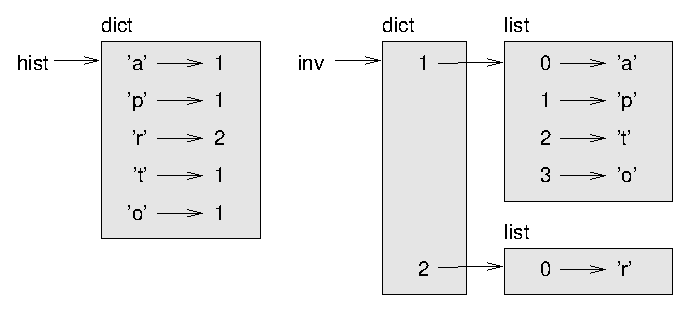
\includegraphics{figs/dict1.eps}}
\afterfig

字典用盒子来表示,类型{\tt dict}在盒子上方,键-值对在盒子里面。
如果值为整型,浮点型或者字符串,通常画在盒子里面,如果是列表,则画在
盒子外面,这样做仅仅是为了保持图的简洁。

列表可以作为字典的关键字值,正如上面的例子演示的。但是,不能作为字典的关键字。请看下面:

\index{TypeError}
\index{exception!TypeError}


\beforeverb
\begin{verbatim}
>>> t = [1, 2, 3]
>>> d = dict()
>>> d[t] = 'oops'
Traceback (most recent call last):
  File "<stdin>", line 1, in ?
TypeError: list objects are unhashable
\end{verbatim}
\afterverb
%

我在之前提到过,字典是用散列方法实现的,这就意味着,关键字必须是可散列的。

\index{hash function 散列函数}
\index{hashable 可散列的}

散列函数,接受一个任何类型的值,返回一个整数。字典使用这些
整数(散列值)存储,查询键-值对。

\index{immutability 不可变性}


如果关键字是不可变的,则一切正常。但是,如果关键字是可变的,比如
列表,麻烦来了。比如,当创建一个键-值对,Python散列关键字,并且
把它存放在相应的位置。如果修改关键字,然后再一次散列,就会散列到
另外一个位置。这种情况下,将会得到两个有着相同键的项,或者可能
无法获取关键字。无论那种情况,字典都不能正常工作。

这就是为什么关键字必须是可散列的,可变数据类型像列表不能作为关键字的原因。最
最简单的解决方式是使用元组,我们在下一章将会遇到。

虽然字典是可变的,不能作为关键字,但是可以作为关键字值。

\begin{ex}
查阅字典方法{\tt setdefault}的文档,用它编写一个更简洁的\verb"invert_dict"。

\index{setdefault method setdefault方法}
\index{method!setdefault}

\end{ex}




\section{备忘录}

如果尝试过\ref{另外一个例子}部分的{\tt fibonacci}函数,可能会
注意到,提供的参数越大,函数运行花费的时间越长。确切地说,运行时间增长
长的很快。

\index{fibonacci function fibonacci函数}
\index{function!fibonacci}

为了一探究竟,看看这个调用图,其中{\tt n = 4}:

\beforefig
\centerline{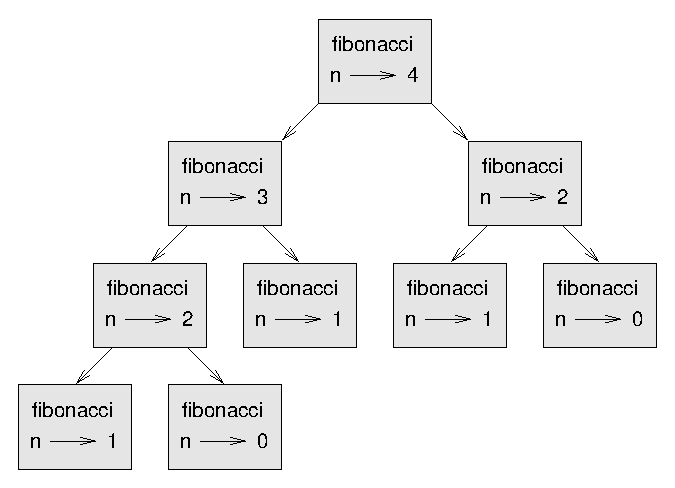
\includegraphics[height=2in]{figs/fibonacci.eps}}
\afterfig


调用图包含了一系列函数框图,每个框图及其调用的函数框图用直线连接。
在调用图的顶部,{\tt n=4}的{\tt fibonacci}调用{\tt n=3} 的
{\tt fibonacci}和{\tt n=2}的{\tt fibonacci}。依次地,{\tt n=3}的{\tt fibonacci}
调用{\tt n=2}和{\tt n=1}的{\tt fibonacci}函数......

\index{function frame 函数框图}
\index{frame}
\index{call graph}

计算一下{\tt fibonacci(0)}和{\tt fibonaci(1)}分别被调用了多少次。可以看出,
这不是解决这个问题的高效方式,并且随着参数变大,效率会更低。

\index{memo 备忘录}

另外一种方法就是跟踪已经被计算的值---把它存储在字典里。存储已经计算的留作后用叫做备忘录\footnote{参考\url{wikipedia.org/wiki/Memoization}。}。下面是使用备忘录实现
的{\tt fibonacci}:

\beforeverb
\begin{verbatim}
known = {0:0, 1:1}

def fibonacci(n):
    if n in known:
        return known[n]

    res = fibonacci(n-1) + fibonacci(n-2)
    known[n] = res
    return res
\end{verbatim}
\afterverb

{\tt known}是一个字典,跟踪我们已经计算出的Fibonacci数字。起始项为:
0映射到0,1映射到1。

无论何时调用{\tt fibonacci},函数检查{\tt known}字典。如果字典包含需要的结果,
函数立刻返回,否则函数计算新值,并把它加入字典,然后返回。

\begin{ex}
运行此版本的{\tt fibonacci}函数和原先的版本,多传递几个参数,然后比较运行的时间。
\end{ex}


\section{全局变量}

\index{global variable 全局变量}
\index{variabl!global 全局}

在以往的例子中,我们在函数外面创建{\tt
	known},所以它属于特殊的框图\verb"__mian__"。
\verb"__main__"内的变量有时称为全局变量,因为任何函数都可以访问它们。不像局部、
变量,在函数返回时销毁,全局变量在函数调用过程中,都是存在的。

\index{flag 标记}

把全局变量作为标记来使用是很常见的,也就是说,布尔变量(“标记”)表明条件是否为真。
比如,有些程序使用{\tt verbose}标记控制输出的层次:

\beforeverb
\begin{verbatim}
verbose = True

def example1():
    if verbose:
        print 'Running example1'
\end{verbatim}
\afterverb

如果试着给一个全局变量重新赋值\footnote{译注:这个地方使用的术语是不准确的。
我们知道Python中使用的是引用,所以不存在赋值,我们可以说重新绑定(rebind)},我们可能会很惊讶。下面的例子跟踪函数是否被
调用:

\index{mutiple assignment 多重赋值}
\index{assignment!multiple 多次}

\beforeverb
\begin{verbatim}
been_called = False

def example2():
    been_called = True         # WRONG
\end{verbatim}
\afterverb

如果运行程序,将会看到\verb"been_called"的值并没有改变。问题在于
{\tt example2}创建了一个新的局部变量\verb"been_called"。局部变量随着函数的终结
而销毁,而对全局变量没有任何影响。

\index{global statement 全局语句}
\index{statement!global 全局}
\index{declaration 声明}

如果要在函数体里为全局变量重新赋值,我们必须在使用前声明全局变量:

\beforeverb
\begin{verbatim}
been_called = False

def example2():
    global been_called 
    been_called = True
\end{verbatim}
\afterverb

{\tt
	global}语句告诉解释器“在这个函数里,当我说\verb"been_called",它就是全局变量,不要创建一个局部变量了。“

\index{update!global variable 全局变量}
\index{global variable!update 更新}

下面是一个更新全局变量值的例子:

\beforeverb
\begin{verbatim}
count = 0

def example3():
    count = count + 1          # WRONG
\end{verbatim}
\afterverb
如果运行它,会得到:

\index{UnboundLocalError}
\index{exception!UnboundLocalError}

\beforeverb
\begin{verbatim}
UnboundLocalError: local variable 'count' referenced before assignment
\end{verbatim}
\afterverb
Python认为{\tt count}是一个局部变量,这也意味着在写之前必须读取它。
解决的方法是,声明{\tt count}为全局变量。

\index{counter 计数器}

beforeverb
\begin{verbatim}
def example3():
    global count
    count += 1
\end{verbatim}
\afterverb
%

如果全局变量是可变的,就可以不声明而修改它:

\index{mutability 可变}

\beforeverb
\begin{verbatim}
known = {0:0, 1:1}

def example4():
    known[2] = 1
\end{verbatim}
\afterverb
%

所以,我们可以添加,删除,替换全局列表和全局字典的元素,但是如果想要
给变量重新赋值,必须声明为全局变量:

\beforeverb
\begin{verbatim}
def example5():
    global known
    known = dict()
\end{verbatim}
\afterverb
%

\section{长整数}

\index{long integer 长整数}
\index{integer!long 长}
\index{type!long 长}

如果计算{\tt fibonacci(50)},我们得到:
\beforeverb
\begin{verbatim}
>>> fibonacci(50)
12586269025L
\end{verbatim}
\afterverb
%

结果尾部的{\tt L}表明该数是一个长整型\footnote{在Python 3.0中,类型{\tt
	long}不存在了;所有整数,即使非常大,也是{\tt int}类型,或者
{\tt long}类型}。

\index{Python 3.0}

{\tt
	int}类型的值是有范围的;长整型值可以是任意大,但是值越大,消耗的空间和时间就越大。

基本数学运算符对长整型适用,{\tt math}模块的函数也如此,所以,一般来说,
{\tt int}的代码也同样适用于{\tt long}。

任何时候,计算结果太大,而整型无法表示的时候,Python自动把结果转换为
长整型:

\beforeverb
\begin{verbatim}
>>> 1000 * 1000
1000000
>>> 100000 * 100000
10000000000L
\end{verbatim}
\afterverb

第一种情况下,结果是{\tt int}型;第二种情况,是{\tt long}型。

\begin{ex}

\index{encryption 加密}
\index{RSA algorithm RSA算法}
\index{algorithm!RSA}

大整数幂是一般公钥加密算法的基础。阅读维基百科中RSA算法页面\footnote{
	\url{wikipedia.org/wiki/RSA}.},然后编写一个函数加密解密信息。
\end{ex}

\section{调试}
\index{debugging 调试}

随着程序数据的增加,通过手动输出并检查数据变得越来越笨拙。下面是关于此种情况
的一些建议:

\begin{description}

\item [缩小输入数据量:]如果可以,尽量减少数据量。比如,如果程序想要读取一个
文本文档,就可以仅仅读取开始的10行,或者其他的你认为比较小的部分。可以修改
文件本身,或者(最好这样)修改程序,让程序只读取文件的前{\tt n}行。

如果出现错误,可以缩小{\tt n}的值,到出现错误的地方,然后逐渐增加它,直到找放到
并更正错误。

\item [检查概要和类型:]不必要输出检查全部数据,考虑输出数据的概要:比如,
字典项的数目或者列表中数字的个数。

一个常见的运行时错误是数据类型错误。调试这种粗无,通常输出值的类型就足够了。

\item [编写自我测试:]有时,可以编写代码自动检查错误。比如,计算列表中数字的
平均数,可以检查结果应该不大于列表的最大元素,不大于最小元素。这个叫做“健康测试”,因为测试发现不健康的结果。


\index{sanity check 健康测试}
\index{consistency check 连贯性测试}

另外一种测试比较两个不同的计算结果,看看他们是否连贯。这叫做“连贯性测试”。

\item
[精巧的打印输出:]格式化调试输出可以更容易发现粗无。参看\ref{factdebug}部分。
{\tt pprint}模块提供{\tt pprint}函数,以人类可读格式显示内置类型。

\index{pretty print 精巧的输出}
\index{pprint module pprint模块}
\index{module!pprint}

\end{description}

再次提醒:花费在搭建“脚手架”的时间越多,用来调试的时间就越少。

\index{scaffolding 脚手架}




\section{术语表}

\begin{description}

\item [dictionary 字典:]键集合到对应值的映射。
\index{dictionary 字典}

\item [key-value pair 键值对:]键--值映射的表示。
\index{key-value pair 键值对}

\item [item 项:]键值对的别名。
\index{item!dictionary 字典}

\item [key 键:] 字典中,键值对的第一个部分。
\index{key 键}

\item [value 关键字值:]字典中,键值对的第二部分。比我们以前使用的单词“值”,
更特殊。
\index{value 关键字值}

\item [implementation 实现:]计算的方式。
\index{implementation 实现}

\item [hashtable 散列表:]实现Python字典的一种算法。
\index{hashtable 散列表}

\item [hash function 散列函数:]计算键位置的函数。
\index{hash function 散列函数}

\item [hashable 散列体:]拥有散列函数的数据类型。不可变类型,像整型,浮点型,
字符串都是散列体;可变类型,比如列表和字典不是。
\index{hashable 散列体}

\item [lookup 查询:]通过关键字查找关键字值的字典操作。
\index{lookup 查询}

\item [reverse lookup 颠倒查询:]通过关键字值查找对应关键字的字典操作。
\index{reverse lookup ,dictionary 颠倒查询,字典}

\item[singleton 独子体]只有一个元素的线性数据结构.
\index{singleton 独子体}

\item [call graph 调用框图:]显示在程序执行时,从调用函数到被调用函数框图的箭
头的图表。
\index{call graph 调用框图}
\index{diagram!call graph 调用框图}

\item [histogram 直方图:]计数器的集合。
index{histogram 直方图}

\item [memo 备忘录:]存储已经计算出的值,留作后用的方法。
\index{memo 备忘录}

\item [global variable 全局变量:]函数体外定义的变量。全局变量可以从任何
函数中访问。
\index{global variable 全局变量}

\item [flag 标记:]表明条件是否成立的布尔变量。
\index{flag 标记}

\item [declaration 声明:] 像{\tt global}语句一样,告诉解释器关于变量的一些
信息。
\index{declaration 声明}

\end{description}



section{练习}

\begin{ex}
\index{duplicate}

如果做了练习\ref{duplicate},已经编写了一个\verb"has_duplicates"函数,它接受
一个列表作为参数,如果有一个对象在列表中出现多次,就返回{\tt True}。

使用字典编写一个更快,更简洁的\verb"has_duplicates"函数。
\end{ex}



\begin{ex}
\label{exroptatepairs}

\index{letter rotation }
\index{rotation!letters}

两个单词,如果“旋转”其中一个可以得到第二个就称为“旋转对”(参看练习\ref{exrotate} \verb"rotate_word")

编写一个程序,读取单词列表,发现所有的旋转对。
\end{ex}



\begin{ex}
\index{Car Talk}
\index{Puzzler 难题}

下面又是一个难题,来自{\em Car
	Talk}\footnote{\url{www.cartalk.com/content/puzzler/transcripts/200717}.}:


\begin{quote}
这个难题来自于Dan O'Leary。他遇到一个常见的由一个音节,五个字母构成的
单词。这个单词具有如下的性质:当移除第一个字母,剩下的字母组成了一个
与原来单词发音形同的单词。如果去掉第二个字母,其他字母不变,剩下的又是
一个同音词。问这个单词是什么?

现在给个不成功的例子。我们随手举个五个字母的单词为例,“wrack“。W-R-A-C-K,之
,比如`wrack with pain' 。如果去掉第一个字母,剩下'R-A-C-K'。就像,`Holy
cow, did you see the rack on that buck!It must have been a nine-pointer!'.
它确实是一个很完美的同音词。如果去掉'r',剩下`wack',它确实是一个单词,但是不
不是同音词了。

但是确实至少有一个符合这个条件的单词---去掉前两个字母中的一个都可以构成
原来单词的同音词。问题是,这个单词是什么?
\end{quote}

\index{homophone 同音词}
\index{reducible world 可化简单词}
\index{word,reducible 单词,可化简}

可以使用练习\ref{wordlist2}的字典,检查字符串是否在字典列表里。

如果要检查两个单词是否是同音词,可以使用卡内基.梅隆大学发音辞典。可以
从这里下载:
\url{www.speech.cs.cmu.edu/cgi-bin/cmudict}或者从这里\url{thinkpython.com/code/c06d} 
也可以下载\url{thinkpython.com/code/pronounce.py},这个模块提供了
函数\verb"read_dictionary",读取发音辞典,返回Python字典,提供了从单词到
对应发音(以字符串表示)的映射。

编写程序,列举能够解决这个难题的所有单词。参看我的解答\url{thinkpython.com/code/homophone.py}。


\end{ex}



































































































































































